\icode{E-MD-SI-L1-261113-005}
国际单位制（缩写SI）定义了米（\qty{}{m}）、秒（\qty{}{s}）等7个基本单位，其他单位均可由物理关系导出。例如，由\qty{}{m}和\qty{}{s}可以导出速度单位\qty{}{m/s}。历史上，曾用“米原器”定义米，用平均太阳日定义秒。但是，以实物或其运动来定义基本单位会受到环境和测量方式等因素的影响，而采用物理常量来定义则可避免这种困扰。1967年用铯-133原子基态的两个超精细能级间跃迁辐射的频率 \(\Delta \nu = \) \qty{9192631770}{Hz}定义秒；1983年用真空中的光速 \(c = \) \qty{299792458}{m/s}定义米。2018年第26届国际计量大会决定，7个基本单位全部用基本物理常量来定义（对应关系如图，例如，秒对应 \(\Delta \nu\)，米对应 \(c\)）。新SI自2019年5月20日（国际计量日）正式实施，这将对科学和技术发展产生深远影响。下列选项不正确的是\paren[]

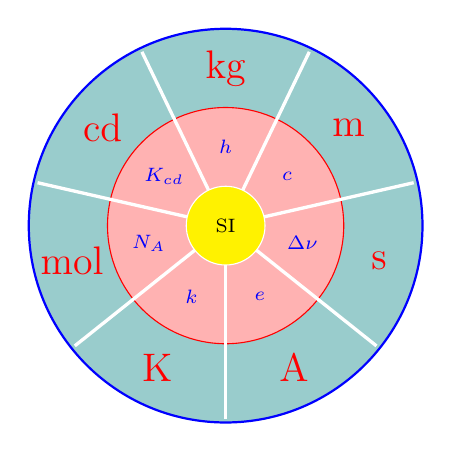
\begin{tikzpicture}[font=\scriptsize]
	\draw[blue,thick,fill=teal!40] (0,0) circle(2.5);
	\draw[red,thin,fill=red!30] (0,0) circle(1.5);
	\foreach \n in {0,1,...,6}
		\draw[white,very thick] (0,0)--({-270/7+\n*360/7}:2.45);
	\foreach \n/\c in {0/s,1/m,2/kg,3/cd,4/mol,5/K,6/A}
		\node[red] at({-90/7+\n*360/7}:2){\Large\qty{}{\c}};
	\foreach \n/\c in {0/{\Delta\nu},1/c,2/h,3/K_{cd},4/N_A,5/k,6/e}
		\node[blue] at({-90/7+\n*360/7}:1){\(\c\)};
	\draw[white,fill=yellow] (0,0) circle(.5);
	\node at(0,0){SI};
\end{tikzpicture}
\begin{choices}
	\item 7个基本单位全部用物理常量定义，保证了基本单位的稳定性
	\item 用真空中的光速 \(c\) (\qty{}{m/s})定义米，因为长度 \(l\) 与速度 \(v\) 存在 \(l = vt\)，而秒已定义
	\item 用基本电荷 \(e\) (\qty{}{C})定义安培(\qty{}{A})，因为电荷量与电流 \(I\) 存在 \(I = q/t\)，而秒已定义
	\item 因为普朗克常量\(h\)(\qty{}{J\cdot s})的单位中没有\qty{}{kg}，所以无法用它来定义质量单位
\end{choices}
\begin{answer}
    D\qquad 提示：
\end{answer}